\chapter{线性代数中的线性方程组}
\section{线性方程组}
包含变量$x_1,x_2,\cdots,x_n$的线性方程:
	\[ a_{1}x_{1}+a_{2}x_{2}+\cdots +a_{n}x_{n}=b \]
其中, $b$与系数$a_{1}$,$a_{2}$,$\cdots$,$a_{n}$是实数或复数, 通常为已知数. n为任意正整数\\[2ex]

线性方程组 -- 由一个或几个包含相同变量$x_1,x_2,\cdots,x_n$的线性方程组成, 如:
\[\begin{array}{r@{\hspace{1.5pt}}l@{\hspace{1.5pt}}r@{\hspace{1.5pt}}l@{\hspace{1.5pt}}r@{\hspace{1.5pt}}l@{\hspace{1.5pt}}r}
	2x_1 & - & x_2 & + & 1.5x_3 & = & 8\\
	x_1  &   &     & - & 4x_3   & = & -7		
\end{array}\]
若线性方程组的方程个数少于未知数个数, 称之为\textbf{欠定方程组}\\
若线性方程组的方程个数多余未知数个数, 称之为\textbf{超定方程组}\\[1ex]

方程组所有可能的解的集合称为线性方程组的\textbf{解集}\\
若两个方程组有相同的解集, 则这两个方程组称为\textbf{等价的}\\[2ex]

\begin{center}
\begin{boxedminipage}{8cm}
线性方程组的解有下列三种情况:\\
1.无解;\\
2.有唯一解;\\
3.有无穷多解.
\end{boxedminipage}
\end{center}\vspace{2ex}

当方程组有唯一解或无穷多解时, 称线性方程组\textbf{相容}; 当方程组无解时, 称线性方程组\textbf{不相容}\\[2ex]

线性方程组
\[\begin{array}{r@{\hspace{1.5pt}}l@{\hspace{1.5pt}}r@{\hspace{1.5pt}}l@{\hspace{1.5pt}}r@{\hspace{1.5pt}}l@{\hspace{1.5pt}}r}
x_1 & - & 2x_2 & + &  x_3 & = & 0\\
	& 	& 2x_2 & - & 8x_3 & = & 8\\
-4x_1 & + & 5x_2 & + & 9x_3 & = & -9
\end{array}\]

线性方程组的\textbf{系数矩阵}
\[\left[\begin{array}{r r r}
	1 & -2 & 1\\
	0 & 2  & -8\\
	-4 & 5 & 9
\end{array}\right]\]

线性方程组的\textbf{增广矩阵}
\[\left[\begin{array}{r r r r}
	1 & -2 & 1 & 0\\
	0 & 2  & -8 & 8\\
	-4 & 5 & 9 & -9
\end{array}\right]\]\\[2ex]

矩阵的\textbf{维数}说明它包含的行数和列数. 如: 当矩阵包含3行4列, 则维数为3$\times$4\\[2ex]

\begin{center}
\begin{boxedminipage}{10cm}
初等行变换:\\
1.倍加变换 - 将某方程替换为它与另一方程倍数的和;\\
2.对换变换 - 交换两个方程的位置;\\
3.倍乘变换 - 方程的所有系数乘以一个非0实数.
\end{boxedminipage}
\end{center}

当其中一个矩阵可以经过一系列初等行变换称为另一个矩阵, 则称两个矩阵为\textbf{行等价的}\\

例1.解下列方程组\\
\[\begin{array}{r@{\hspace{1.5pt}}l@{\hspace{1.5pt}}r@{\hspace{1.5pt}}l@{\hspace{1.5pt}}r@{\hspace{1.5pt}}l@{\hspace{1.5pt}}r}
	x_1 & - & 2x_2 & + & x_3 & = & 0\\
	& & 2x_2 & - & 8x_3 & = & 8\\
	-4x_1 & + & 5x_2 & + & 9x_3 & = & -9
\end{array}\]
推导过程:\\
增广矩阵:\\
\[\left[\begin{array}{r r r r}
	1 & -2 & 1 & 0\\
	0 & 2 & -8 & 8\\
	5 & 0 & -5 & 10
\end{array}\right]\]
1)\ding{174}-5\ding{172}, 得:\\
\[\left[\begin{array}{r r r r r} 
	1 & -2 & 1 & 0\\
	0 & 2 & -8 & 8\\
	0 & 10 & -10 & 10
\end{array}\right]\]
2)$\frac{1}{2}$\ding{173}, 得:\\
\[\left[\begin{array}{r r r r r} 
	1 & -2 & 1 & 0\\
	0 & 1 & -4 & 4\\
	0 & 10 & -10 & 10
\end{array}\right]\]
3)\ding{174}-10\ding{172}, 得:\\
\[\left[\begin{array}{r r r r r} 
	1 & -2 & 1 & 0\\
	0 & 1 & -4 & 4\\
	0 & 0 & 30 & -30
\end{array}\right]\]
4)$\frac{1}{30}$\ding{174}, 得:\\
\[\left[\begin{array}{r r r r r} 
	1 & -2 & 1 & 0\\
	0 & 1 & -4 & 4\\
	0 & 0 & 1 & -1
\end{array}\right]\]
5)\ding{173}+4\ding{174}, 得:\\
\[\left[\begin{array}{r r r r r} 
	1 & -2 & 1 & 0\\
	0 & 1 & 0 & 0\\
	0 & 0 & 1 & -1
\end{array}\right]\]
6)\ding{172}-\ding{174}, 得:\\
\[\left[\begin{array}{r r r r r} 
	1 & -2 & 0 & 1\\
	0 & 1 & 0 & 0\\
	0 & 0 & 1 & -1
\end{array}\right]\]
7)\ding{172}+2\ding{173}, 得:\\
\[\left[\begin{array}{r r r r r} 
	1 & 0 & 0 & 1\\
	0 & 1 & 0 & 0\\
	0 & 0 & 1 & -1
\end{array}\right]\]
方程组的解:(1,0,-1)\\[1ex]

例2.确定方程组是否相容\\
\[\begin{array}{r@{\hspace{1.5pt}}l@{\hspace{1.5pt}}r@{\hspace{1.5pt}}l@{\hspace{1.5pt}}r@{\hspace{1.5pt}}l@{\hspace{1.5pt}}r}
	& & x_2 & - & 4x_3 & = & 8\\
	2x_1& - & 3x_2 & + & 2x_3 & = & 1\\
	4x_1 & - & 8x_2 & + & 12x_3 & = & 1
\end{array}\]
推导过程:\\
增广矩阵:\\
\[\left[\begin{array}{r r r r}
	0 & 1 & -4 & 8\\
	2 & -3 & 2 & 1\\
	4 & -8 & 12 & 1
\end{array}\right]\]
1)\ding{172}$\rightleftharpoons$\ding{173}, 得:\\
\[\left[\begin{array}{r r r r}
	2 & -3 & 2 & 1\\
	0 & 1 & -4 & 8\\
	4 & -8 & 12 & 1
\end{array}\right]\]
2)\ding{174}-2\ding{172}, 得:\\
\[\left[\begin{array}{r r r r}
	2 & -3 & 2 & 1\\
	0 & 1 & -4 & 8\\
	0 & -2 & 8 & -1
\end{array}\right]\]
3)\ding{174}+2\ding{173}, 得:\\
\[\left[\begin{array}{r r r r}
	2 & -3 & 2 & 1\\
	0 & 1 & -4 & 8\\
	0 & 0 & 0 & 15
\end{array}\right]\]
方程组不相容\\[1ex]

\begin{center}
\framebox{若两个线性方程组的增广矩阵是行等价的, 则它们具有相同的解集}
\end{center}
\newpage

\section{行化简与阶梯形矩阵}
非零行(列): 矩阵中至少包含一个非零元素的行(列)\\
先导元素: 该行最左边的非零元素\\
\begin{definition}
一个矩阵称为阶梯形, 若它有以下三个性质:\\
1.所有非零行在零行之上;\\
2.某一行先导元素的列位于上一行先导元素的右边;\\
3.某一先导元素所在列下方元素都是零;\\
若还满足以下性质, 则称为简化阶梯形:\\
4.每一非零行的先导元素是1;\\
5.每一先导元素是该元素所在列的唯一非零元素.
\end{definition}\vspace{2ex}

\begin{TheoremTwo}[简化阶梯形矩阵的唯一性]
每个矩阵行等价于唯一的简化阶梯形矩阵.
\end{TheoremTwo}\vspace{2ex}

若矩阵A行等价于阶梯形矩阵U, 则称U为A的\textbf{阶梯形}; 若U是简化阶梯形, 则称U为A的\textbf{简化阶梯形}. \\
RREF(Reduced Row-Echelon Form): 简化阶梯形\\
REF(Row-Echelon Form): 阶梯形\\[2ex]

\begin{definition}
矩阵A中的{\heiti 主元位置}是A中对应于它的阶梯形中先导元素的位置.{\heiti 主元列}是A中含有主元位置的列.
\end{definition}\vspace{2ex}

例1.将下列矩阵利用行变换转化为阶梯型
\[A=\left[
\begin{array}{r r r r r}
	0 & -3 & -6 & 4 & 9\\
	-1 & -2 & -1 & 3 & 1\\
	-2 & -3 & 0 & 3 & -1\\
	1 & 4 & 5 & -9 & -7
\end{array}
\right]\]
推导过程:\\
1)\ding{172}$\rightleftharpoons$\ding{175}, 得:\\
\[\left[
\begin{array}{r r r r r}
	1 & 4 & 5 & -9 & -7\\
	-1 & -2 & -1 & 3 & 1\\
	-2 & -3 & 0 & 3 & -1\\
	0 & -3 & -6 & 4 & 9
\end{array}
\right]\]
2)\ding{173}+\ding{172}, 得:\\
\[\left[
\begin{array}{r r r r r}
	1 & 4 & 5 & -9 & -7\\
	0 & 2 & 4 & -6 & -6\\
	-2 & -3 & 0 & 3 & -1\\
	0 & -3 & -6 & 4 & 9
\end{array}
\right]\]
3)\ding{174}+2\ding{172}, 得:\\
\[\left[
\begin{array}{r r r r r}
	1 & 4 & 5 & -9 & -7\\
	0 & 2 & 4 & -6 & -6\\
	0 & 5 & 10 & -15 & -15\\
	0 & -3 & -6 & 4 & 9
\end{array}
\right]\]
4)\ding{174}-$\frac{5}{2}$\ding{173}, 得:\\
\[\left[
\begin{array}{r r r r r}
	1 & 4 & 5 & -9 & -7\\
	0 & 2 & 4 & -6 & -6\\
	0 & 0 & 0 & 0 & 0\\
	0 & -3 & -6 & 4 & 9
\end{array}
\right]\]
5)\ding{174}$\rightleftharpoons$\ding{175}, 得:\\
\[\left[
\begin{array}{r r r r r}
	1 & 4 & 5 & -9 & -7\\
	0 & 2 & 4 & -6 & -6\\
	0 & -3 & -6 & 4 & 9\\
	0 & 0 & 0 & 0 & 0
\end{array}
\right]\]


基本变量: 位于主元列的变量\\
自由变量: 位于非主元列的变量\\[2ex]

\begin{TheoremTwo}[存在与唯一性定理]
线性方程组相容的充要条件是增广矩阵的最右列不是主元列. 也就是说, 增广矩阵的阶梯形没有形如
	\[[0\ \cdots\ 0\ b], b\neq 0\]
的行. 若线性方程组相容, 则它的解集可能有两种情形:\\
1)当没有自由变量时, 有唯一解;\\
2)若至少有一个自由变量, 则有无穷多解.
\end{TheoremTwo}\vspace{2ex}

应用行化简算法解线性方程组:\\
1.写出方程组的增广矩阵\\
2.应用行化简算法把增广矩阵化为阶梯形, 确定方程组是否相容, 如果没有解则停止; 否则进行下一步\\
3.继续行化简算法得到它的简化阶梯形\\
4.写出简化阶梯形矩阵对应的方程组\\
5.将每个非零方程改写为使用自由变量表示基本变量的形式
\newpage

\section{向量方程}
仅含一列的矩阵称为列向量, 简称为向量. 包含两个元素得向量如下:
\[u=\left[\begin{array}{r}
	3\\
	-1
\end{array}\right] \text{\quad or\quad} u=(3, -1)\]\\[1ex]
所有两个元素的向量表示为$\mathbb{R}^2$, $\mathbb{R}$表示向量中的元素为实数, 2表示向量包含两个元素\\[1ex]

向量相等:\\
两个向量相等当且仅当其对应元素相等\\[1ex]

向量加法:\\
将向量的对应元素相加
\begin{equation*}
\left[\begin{array}{c}
	1\\
	-2
\end{array}\right]
+
\left[\begin{array}{c}
	2\\
	5
\end{array}\right]
=
\left[\begin{array}{c}
	1+2\\
	-2+5
\end{array}\right]
=
\left[\begin{array}{c}
	3\\
	3
\end{array}\right]
\end{equation*}

标量乘法:\\
将向量的元素乘以系数\\
\indent 若$u=\left[\begin{array}{c}3\\-1\end{array}\right]$, $c=5$, 则:
\[cu=5\left[\begin{array}{c}3\\-1\end{array}\right]=\left[\begin{array}{c}15\\-5\end{array}\right]\]

向量$\left[\begin{array}{r}x\\y\end{array}\right]$的几何含义: 由原点(0,0)指向点(x,y)的有向线段\\[2ex]

\begin{law}[向量加法的平行四边形法则]\ \\
若$\mathbb{R}^2$中向量$\mathbf{u}$和$\mathbf{v}$用平面上的点表示, 则$\mathbf{u+v}$对应于以$\mathbf{u}$,$\mathbf{0}$和$\mathbf{v}$为三个顶点的平行四边形的第4个顶点, 如图.\\[2ex]
\begin{center}
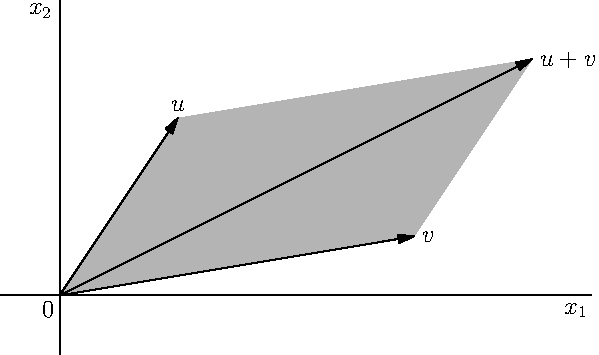
\includegraphics{vector_addition.pdf}
\end{center}
\end{law}\vspace{3ex}

所有元素都是零的向量称为\textbf{零向量}, 用\textbf{0}表示(\textbf{0}中元素的个数可由上下文确定)\\[2ex]

\begin{law}[$\mathbb{R}^n$中向量的代数性质]\ \\
对$\mathbb{R}^n$中一切向量$\mathbf{u}$,$\mathbf{v}$,$\mathbf{w}$以及标量$c$和$d$:
\begin{equation*}
\begin{array}{l@{}c@{}l l l@{}c@{}l l}
( & i & ) & \mathbf{u}+\mathbf{v}=\mathbf{v}+\mathbf{u} & ( & v & ) & c(\mathbf{u}+\mathbf{v})=c\mathbf{u}+c\mathbf{v}\\
( & ii & ) & (\mathbf{u}+\mathbf{v})+\mathbf{w}=\mathbf{u}+(\mathbf{v}+\mathbf{w}) & ( & vi & ) & (c+d)\mathbf{u}=c\mathbf{u}+d\mathbf{u}\\
( & iii & ) & \mathbf{u}+\mathbf{0}=\mathbf{0}+\mathbf{u}=\mathbf{u} & ( & vii & ) & c(d\mathbf{u})=(cd)\mathbf{u}\\
( & iv & ) & \mathbf{u}+(-\mathbf{u})=-\mathbf{u}+\mathbf{u}=\mathbf{0} & ( & viii & ) & 1\mathbf{u}=\mathbf{u}
\end{array}
\end{equation*}
\end{law}\vspace{2ex}

给定$\mathbb{R}^n$中向量$\mathbf{v}_1$,$\mathbf{v}_2$,$\cdots$,$\mathbf{v}_p$和标量$c_1$,$c_2$,$\cdots$,$c_p$, 向量
	\[\mathbf{y}=c_1\mathbf{v}_1+\cdots+c_p\mathbf{v}_p\]
称为向量$\mathbf{v}_1$,$\mathbf{v}_2$,$\cdots$,$\mathbf{v}_p$以$c_1$,$c_2$,$\cdots$,$c_p$为\textbf{权}的\textbf{线性组合}.\\[2ex]

\framebox{
\begin{minipage}{\linewidth}
向量方程
\[x_1\mathbf{a}_1+x_2\mathbf{a}_2+\cdots+x_n\mathbf{a}_n=\mathbf{b}\]
和增广矩阵为
\begin{equation}
[\mathbf{a}_1\quad\mathbf{a}_2\quad\cdots\quad\mathbf{a}_n\quad\mathbf{b}]\label{matrix:eq_01}
\end{equation}
的线性方程组有相同的解集. 特别地, $\mathbf{b}$可表示为$\mathbf{a}_1$,$\mathbf{a}_2$,$\cdots$,$\mathbf{a}_n$的线性组合当且仅当对应于\eqref{matrix:eq_01}式的线性方程组有解.
\end{minipage}}\\[4ex]

\begin{definition}
若$\mathbf{v}_1$,$\mathbf{v}_2$,$\cdots$,$\mathbf{v}_p$是$\mathbb{R}^n$中的向量, 则$\mathbf{v}_1$,$\mathbf{v}_2$,$\cdots$,$\mathbf{v}_p$的所有线性组合所成的组合用记号$\Span\{\mathbf{v}_1$,$\mathbf{v}_2$,$\cdots$,$\mathbf{v}_p\}$表示, 称为由$\mathbf{v}_1$,$\mathbf{v}_2$,$\cdots$,$\mathbf{v}_p$所\textbf{生成}(或\textbf{张成})\textbf{的$\mathbb{R}^n$的子集}. 也就是说, $\Span\{\mathbf{v}_1$,$\mathbf{v}_2$,$\cdots$,$\mathbf{v}_p\}$是所有形如
	\[c_1\mathbf{v}_1+c_2\mathbf{v}_2+\cdots+c_p\mathbf{v}_p\]
的向量的集合, 其中$c_1$,$c_2$,$\cdots$,$c_p$为标量.\\[2ex]
\end{definition}\vspace{4ex}

\section{矩阵方程$A\mathbf{x}=\mathbf{b}$}
\begin{definition}
若$A$是$m\times n$矩阵, 它的各列为$\bm{a}_1$,$\cdots$,$\bm{a}_n$. 若$\bm{x}$是$\mathbb{R}^n$中的向量, 则\textbf{$A$与$\bm{x}$的积}(记为$A\bm{x}$)就是\textbf{$A$的各列以$\bm{x}$中对应元素为权的线性组合}, 即
	\[A\bm{x}=[\bm{a}_1\ \bm{a}_2\ \cdots\ \bm{a}_n]\left[\begin{array}{c}x_1\\x_2\\\vdots\\x_n\end{array}\right]=x_1\bm{a}_1+x_2\bm{a}_2+\cdots+x_n\bm{a}_n\]
注意$A\bm{x}$仅当$A$的列数等于$\bm{x}$中的元素个数时才有意义.\\[2ex]
\end{definition}

\begin{TheoremOne}
若$A$是$m\times n$矩阵, 它的各列为$\bm{a}_1$,$\cdots$,$\bm{a}_n$, 而$\bm{b}$属于$\mathbb{R}^n$, 则矩阵方程
\[A\bm{x}=\bm{b}\]
与向量方程
\[x_1\bm{a}_1+x_2\bm{a}_2+\cdots+x_n\bm{a}_n=\bm{b}\]
有相同的解集. 它又与增广矩阵为
\[[\bm{a}_1\ \bm{a}_2\ \cdots\ \bm{a}_n\ \bm{b}]\]
的线性方程组有相同的解集.\\[2ex]
\end{TheoremOne}

\begin{center}
\framebox{
方程$Ax=b$有解当且仅当$b$是$A$的各列的线性组合
}
\end{center}\vspace{4ex}

\begin{TheoremOne}
设$A$是$m\times n$矩阵, 则下列命题是逻辑上等价的. 也就是说, 对某个$A$, 它们都成立或者都不成立.\\
\begin{tabular}{l@{\,}l}
a. & 对$\mathbb{R}^m$中每个$\bm{b}$, 方程$A\bm{x}=\bm{b}$有解.\\
b. & $\mathbb{R}^m$中的每个$\bm{b}$都是$A$的列的一个线性组合.\\
c. & $A$的各列生成$\mathbb{R}^m$.\\
d. & $A$在每一行都有一个主元位置.\\[2ex]
\end{tabular}
\end{TheoremOne}\vspace{2ex}

\begin{law}[计算$A\bm{x}$的行---向量规则]\ \\
若乘积$A\bm{x}$有定义, 则$A\bm{x}$中的第$i$个元素是$A$的第$i$行元素与$\bm{x}$的相应元素乘积之和.
\end{law}\vspace{2ex}

例1.\\
$\displaystyle a.\left[\begin{array}{r r r}
	1 & 2 & -1\\
	0 & -5 & 3
    \end{array}\right]
    \left[\begin{array}{r}
        4\\
	3\\
	7
    \end{array}\right]=
    \left[\begin{array}{r}
        1\cdot4+2\cdot3+(-1)\cdot7\\
	0\cdot4+(-5)\cdot3+3\cdot7
    \end{array}\right]=
    \left[\begin{array}{r}
        3\\
	6
    \end{array}\right]$\\[2ex]

$\displaystyle b.\left[\begin{array}{r r r}
	1 & 0 & 0\\
	0 & 1 & 0\\
	0 & 0 & 1
    \end{array}\right]
    \left[\begin{array}{r}
        r\\
	s\\
	t
    \end{array}\right]=
    \left[\begin{array}{r}
        1\cdot r+0\cdot s+0\cdot t\\
	0\cdot r+1\cdot s+0\cdot t\\
	0\cdot r+0\cdot s+1\cdot t
    \end{array}\right]=
    \left[\begin{array}{r}
	r\\
	s\\
	t
    \end{array}\right]$\\[2ex]

矩阵的主对角线上元素为1, 其他位置上元素为0, 这个矩阵称为\textbf{单位矩阵}, 并记为$I$.\\
如果矩阵为$n\times n$单位矩阵, 记为$I_n$.\\[2ex]

\begin{TheoremOne}
若$A$是$m\times n$矩阵, $\bm{u}$和$\bm{v}$是$\mathbb{R}^n$中向量, c是标量, 则\\
\begin{tabular}{l@{\,}l}
a. & $A(\bm{u}+\bm{v})=A\bm{u}+A\bm{v}$\\
b. & $A(c\bm{u})=c(A\bm{u})$
\end{tabular}
\end{TheoremOne}\vspace{6ex}

\section{线性方程组的解集}
若线性方程组可写成
\[A\bm{x}=\bm{0}\]
的形式, 则称为\textbf{齐次线性方程组}. 其中, $A$是$m\times n$矩阵, $\bm{0}$是$\mathbb{R}^m$中的零向量.\\
齐次线性方程组至少有一个解, 即$\bm{x}=\bm{0}$($\mathbb{R}^n$中的零向量), 这个解称为它的\textbf{平凡解}.\\
如果有一个非零向量$\bm{x}$, 满足$A\bm{x}=\bm{0}$, 这个解称为它的\textbf{非平凡解}.\\[2ex]

\begin{law}
齐次方程$A\bm{x}=\bm{0}$有非平凡解当且仅当方程至少有一个自由变量.
\end{law}\vspace{2ex}

$\bm{x}=s\bm{u}+t\bm{v}$为$A\bm{x}=\bm{0}$的\textbf{参数向量形式}, 并称之为\textbf{参数向量方程}. 其中, $s$,$t$为自由变量\\
$\bm{x}=\bm{p}+t\bm{v}$为$A\bm{x}=\bm{b}$的\textbf{参数向量形式}, 并称之为\textbf{参数向量方程}. 其中, $t$为自由变量\\[1ex]

例.\\
$x_1=0.3x_2+0.2x_3$\\[1ex]
$\bm{x}=
\left[\begin{array}{l}
x_1\\
x_2\\
x_3
\end{array}\right]=
\left[\begin{array}{c}
0.3x_2+0.2x_3\\
x_2\\
x_3
\end{array}\right]=
\left[\begin{array}{r}
0.3x_2\\
x_2\\
0
\end{array}\right]+\left[\begin{array}{r}
0.2x_3\\
0\\
x_3
\end{array}\right]\\
\phantom{\bm{x}}=x_2\left[\begin{array}{r}
0.3\\
1\\
0
\end{array}\right]+x_3\left[\begin{array}{r}
0.2\\
0\\
1
\end{array}\right]
$\\[2ex]
因此, $A\bm{x}=\bm{b}$的解集是一条通过$\bm{p}$而平行于$A\bm{x}=\bm{0}$的解集的直线. 也称为将$\bm{v}$沿着$\bm{p}$进行直线移动.\\[2ex]

\begin{TheoremOne}
设方程$A\bm{x}=\bm{b}$对某个$\bm{b}$是相容的, $\bm{p}$为一个特解, 则$A\bm{x}=\bm{b}$的解集是所有形如$\bm{w}=\bm{p}+\bm{v}_h$的向量的集, 其中$\bm{v}_h$时齐次方程$A\bm{x}=\bm{b}$的任意一个解.
\end{TheoremOne}\vspace{3ex}

\begin{law}[把(相容方程组的)解集表示成参数向量形式]\ \\
1.把增广矩阵简化为简化阶梯形.\\
2.把每个基本变量用自由变量表示.\\
3.把一般解$\bm{x}$表示成向量, 如果有自由变量, 其元素依赖于自由变量.\\
4.把$\bm{x}$分解为向量(元素为常数)的线性组合, 用自由变量作为参数.
\end{law}\vspace{4ex}

\section{线性方程组的应用}
1.经济学 - 部分的收支平衡\\[1ex]
例1.\\
假设一个经济体系由煤炭、电力和钢铁三个部门组成, 各部门之间的分配如下所示, 其中每一列中的数表示该部门总产出所占的比例. 设$p_C$,$p_E$,$p_S$分别为煤炭、电力和钢铁部门年度总产出的价格, 求出使每个部门收支平衡的产值.
\begin{table}[H]
\begin{tabular}{>{\centering\arraybackslash}p{0.2\textwidth}|>{\centering\arraybackslash}p{0.2\textwidth}|>{\centering\arraybackslash}p{0.2\textwidth}|>{\centering\arraybackslash}p{0.25\textwidth}}
    \hline
    \multicolumn{3}{c|}{\ziju{0.2}部门的产出分配} & \multirow{2}*{\ziju{0.8}采购部门}\\\cline{1-3}
    \ziju{1.5}煤炭 & \ziju{1.5}电力  & \ziju{1.5}钢铁 & \\\hline
    0.0 & 0.4 & 0.6 & 煤炭\\\hline
    0.6 & 0.1 & 0.2 & 电力\\\hline
    0.4 & 0.5 & 0.2 & 钢铁\\\hline
\end{tabular}
\caption{一个简单的经济问题}
\end{table}
解:\\
\[
    \left\{\begin{array}{r@{\hspace{2pt}}r@{\hspace{2pt}}r@{\hspace{2pt}}r@{\hspace{2pt}}r@{\hspace{2pt}}r@{\hspace{2pt}}r}
	p_C    & - & 0.4p_E & - & 0.6p_S & = & 0\\
	0.6p_C & - & 0.9p_E & + & 0.2p_S & = & 0\\
	0.4p_C & + & 0.5p_E & - & 0.8p_S & = & 0
    \end{array}\right.
\]
增广矩阵为:\\
$\displaystyle\left[\begin{array}{r r r r}
    5 & -2 & -3 & 0\\
    6 & -9 & 2 & 0\\
    4 & 5 & -8 & 0
\end{array}\right]$\\[1ex]

化简矩阵步骤:\\
1.5\ding{173}-6\ding{172}, 得:\\
$\displaystyle\left[\begin{array}{r r r r}
    5 & -2 & -3 & 0\\
    0 & -33 & 28 & 0\\
    4 & 5 & -8 & 0
\end{array}\right]$\\

2.5\ding{174}-4\ding{172}, 得:\\
$\displaystyle\left[\begin{array}{r r r r}
    5 & -2 & -3 & 0\\
    0 & -33 & 28 & 0\\
    0 & 33 & -28 & 0
\end{array}\right]$\\

3.\ding{174}+\ding{173}, 得:\\
$\displaystyle\left[\begin{array}{r r r r}
    5 & -2 & -3 & 0\\
    0 & -33 & 28 & 0\\
    0 & 0 & 0 & 0
\end{array}\right]$\\

4.33\ding{172}-2\ding{173}, 得:\\
$\displaystyle\left[\begin{array}{r r r r}
    165 & 0 & -155 & 0\\
    0 & -33 & 28 & 0\\
    0 & 0 & 0 & 0
\end{array}\right]$\\

5.化简主元, 得:\\
$\displaystyle\left[\begin{array}{r r r r}
    1 & 0 & -0.94 & 0\\
    0 & 1 & -0.85 & 0\\
    0 & 0 & 0 & 0
\end{array}\right]$\\[2ex]

2.化学式 - 等号两边原子守恒\\[2ex]

3.网络流 - 节点的进/出流量恒等\\
例2. 如下图, 该网络是巴尔的摩市区一些单行道在一个下午早些时候(以每小时车辆数目计算)的交通流量. 计算该网络的车流量\\
\begin{figure}[H]
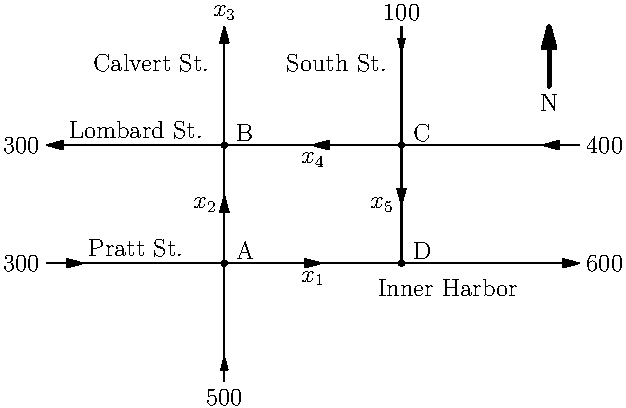
\includegraphics{traffic}
\caption{巴尔的摩道路}
\end{figure}
由每个路口的流量与总流量, 可得到方程组:
\[
\left\{\begin{array}{r r r r r r r r r r r}
    x_1 & + & x_2 & & & & & & & = & 800\\
    & & x_2 & - & x_3 & + & x_4 & & & = & 300\\
    & & & & x_3 & & & & & = & 400\\
    & & & & & & x_4 & + & x_5 & = & 500\\
    x_1 & & & & & & & + & x_5 & = & 600
\end{array}\right.
\]
对应的增广矩阵:
\[
\left[\begin{array}{r r r r r r}
    1 & 1 & 0 & 0 & 0 & 800\\
    0 & 1 & -1 & 1 & 0 & 300\\
    0 & 0 & 1 & 0 & 0 & 400\\
    0 & 0 & 0 & 1 & 1 & 500\\
    1 & 0 & 0 & 0 & 1 & 600
\end{array}\right]
\]
化简后的结果:
\[
\left[\begin{array}{r r r r r r}
    1 & 0 & 0 & 0 & 1 & 600\\
    0 & 1 & 0 & 0 & -1 & 200\\
    0 & 0 & 1 & 0 & 0 & 400\\
    0 & 0 & 0 & 1 & 1 & 500
\end{array}\right]
\]
所以
\[
x=\left\{\begin{array}{c}
    x_1\\
    x_2\\
    x_3\\
    x_4\\
    x_5
\end{array}\right.=\left[\begin{array}{r@{\hspace{1pt}}r@{\hspace{1pt}}r}
    600 & - & x_5\\
    200 & + & x_5\\
    400 & &\\
    500 & - & x_5\\
    & & x_5
\end{array}\right]=\left[\begin{array}{r}
    600\\
    200\\
    400\\
    500\\
    0
\end{array}\right]+\left[\begin{array}{r}
    -1\\
    1\\
    0\\
    -1\\
    1
\end{array}\right]x_5
\]\\[4ex]

\section{线性无关}
\begin{definition}
$\mathbb{R}^n$中一组向量$\{\bm{v}_1$,$\cdots$,$\bm{v}_p\}$称为\textbf{线性无关}的, 若向量方程
\[x_1\bm{v}_1+x_2\bm{v}_2+\cdots+x_p\bm{v}_p=\bm{0}\]
仅有平凡解. 向量组(集)$\{\bm{v}_1$,$\cdots$,$\bm{v}_p\}$称为\textbf{线性相关}的, 若存在不全为零的权$c_1$,$\cdots$,$c_p$, 使
\[c_1\bm{v}_1+c_2\bm{v}_2+\cdots+c_p\bm{v}_p=\bm{0}\]
\end{definition}\vspace{2ex}

\begin{law}
矩阵$A$的各列线性无关, 当且仅当方程$A\bm{x}=\bm{0}$仅有平凡解.
\end{law}\vspace{2ex}

例1.\\
确定矩阵$\displaystyle A=\left[\begin{array}{r r r}
    0 & 1 & 4\\
    1 & 2 & -1\\
    5 & 8 & 0
\end{array}\right]$的各列是否线性无关\\
解.\\
将增广矩阵进行化简:\\
\[
\left[\begin{array}{r r r r}
    0 & 1 & 4 & 0\\
    1 & 2 & -1 & 0\\
    5 & 8 & 0 & 0
\end{array}\right]\sim\left[\begin{array}{r r r r}
    1 & 2 & -1 & 0\\
    0 & 1 & 4 & 0\\
    0 & -2 & 5 & 0
\end{array}\right]\sim\left[\begin{array}{r r r r}
    1 & 2 & -1 & 0\\
    0 & 1 & 4 & 0\\
    0 & 0 & 13 & 0
\end{array}\right]
\]
由于方程没有自由变量, 因此方程$A\bm{x}=\bm{0}$只有平凡解.\\[2ex]

\begin{law}
两个向量的集合$\{\bm{v}_1$,$\bm{v}_2\}$线性相关, 当且仅当其中一个向量是另一个向量的倍数. 这个集合线性无关, 当且仅当其中任一个向量都不是另一个向量的倍数.
\end{law}\vspace{4ex}

\begin{TheoremTwo}[线性相关集的特征]
两个或更多个向量的集合$S=\{\bm{v}_1,\cdots,\bm{v}_p\}$线性相关, 当且仅当S中至少有一个向量是其他向量的线性组合. 事实上, 若S线性相关, 且$\bm{v}_1\neq\bm{0}$, 则某个$\bm{v}_j$$(j>1)$是它前面向量$\bm{v}_1$,$\cdots$,$\bm{v}_{j-1}$的线性组合.
\end{TheoremTwo}\vspace{4ex}

\begin{TheoremOne}
若一个向量组的向量个数超过每个向量的元素个数, 那么这个向量组线性相关. 就是说, $\mathbb{R}^n$中任意向量组$\{\bm{v}_1$,$\cdots$,$\bm{v}_p\}$当$p>n$时线性相关.
\end{TheoremOne}\vspace{4ex}

\begin{TheoremOne}
若$\mathbb{R}^n$中向量组$S=\{\bm{v}_1,\cdots,\bm{v}_p\}$包含零向量, 则它线性相关.
\end{TheoremOne}\vspace{4ex}

\section{线性变换介绍}
由$\bm{x}$到$A\bm{x}$的对应是由一个向量集到另一个向量集的函数\\[2ex]

\begin{definition}
变换(或映射)$T$称为\textbf{线性}的, 若\\
\begin{tabular}{l@{}c@{}l@{\hspace{2pt}}l}
$($ & i & $)$ & 对$T$的定义域中一切$\bm{u}$,$\bm{v}$,$T(\bm{u}+\bm{v})=T(\bm{u})+T(\bm{v})$.\\
$($ & ii & $)$ & 对$T$的定义域中的一切$\bm{u}$和数$c$, $T(c\bm{u})=cT(\bm{u})$.
\end{tabular}
\end{definition}\vspace{4ex}

\begin{law}
若T是线性变换, 则
\[T(\bm{0})=\bm{0}\]
且对$T$的定义域中一切向量$\bm{u}$和$\bm{v}$以及数$c$和$d$, 有:
\[T(c\bm{u}+d\bm{v})=cT(\bm{u})+dT(\bm{v})\]
\end{law}\vspace{2ex}

给定数$r$, 定义$T:\mathbb{R}^2\rightarrow\mathbb{R}^2$为$T(\bm{x})=r\bm{x}$. 当$0\leqslant r\leqslant 1$时, $T$称为\textbf{压缩变换}; 当$r>1$时, $T$称为\textbf{拉伸变换}.\\[4ex]

\section{线性变换的矩阵}
\begin{TheoremOne}
设$T$:$\mathbb{R}^n\rightarrow\mathbb{R}^m$为线性变换, 则存在唯一的矩阵$A$, 使得对$\mathbb{R}^n$中一切$\bm{x}$, 有
\[T(\bm{x})=A\bm{x}\]
事实上, $A$是$m\times n$矩阵, 它的第$j$列是向量$T(\bm{e}_j)$, 其中$\bm{e}_j$是$\mathbb{R}^n$中单位矩阵$\bm{I}_n$的第$j$列:
\[A=[T(\bm{e}_1)\ \cdots\ T(\bm{e}_n)]\]
\end{TheoremOne}\vspace{4ex}

\begin{definition}
映射$T$:$\mathbb{R}^n\rightarrow\mathbb{R}^m$称为到$\mathbb{R}^m$上的映射, 若$\mathbb{R}^m$中每个$\bm{b}$是$\mathbb{R}^n$中至少一个$\bm{x}$的像(也称为\textbf{满射}).
\end{definition}\vspace{4ex}

\begin{definition}
映射$T$:$\mathbb{R}^n\rightarrow\mathbb{R}^m$称为\textbf{一对一映射}(或1:1), 若$\mathbb{R}^m$中每个$\bm{b}$是$\mathbb{R}^n$中至多一个$\bm{x}$的像(也称为\text{单射}).
\end{definition}\vspace{4ex}

\begin{TheoremOne}
设$T$:$\mathbb{R}^n\rightarrow\mathbb{R}^m$为线性变换, 则$T$是一对一的当且仅当方程$A\bm{x}=\bm{0}$仅有平凡解.
\end{TheoremOne}\vspace{4ex}

\begin{TheoremOne}
设$T$:$\mathbb{R}^n\rightarrow\mathbb{R}^m$是线性变换, 设$A$为$T$的标准矩阵, 则\\
\begin{tabular}{l@{\ }l}
a. & $T$把$\mathbb{R}^n$映上到$\mathbb{R}^m$, 当且仅当$A$的列生成$\mathbb{R}^m$.\\
b. & $T$是一对一的, 当且仅当$A$的列线性无关.
\end{tabular}
\end{TheoremOne}\vspace{2ex}

\begin{longtable}{>{\raggedright}m{0.35\linewidth}>{\centering}m{0.35\linewidth}>{\centering\arraybackslash}m{0.25\linewidth}}
\hline
变换名称 & 变换图像 & 标准矩阵\\\hline
旋转 & \raisebox{0pt}[4.2cm][0.2cm]{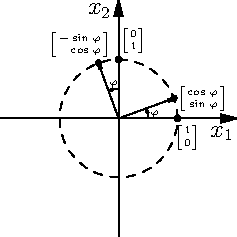
\includegraphics[totalheight=4cm]{rotate}} & $\left[\begin{array}{r r}\cos\varphi & -\sin\varphi\\ \sin\varphi & \cos\varphi\end{array}\right]$\\\hline
关于$x$轴对称 & \raisebox{0pt}[4.2cm][0.2cm]{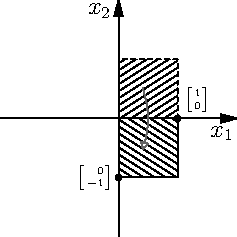
\includegraphics[totalheight=4cm]{symmetry_01}} & $\left[\begin{array}{r r} 1 & 0\\ 0 & -1\end{array}\right]$\\\hline
关于$y$轴对称 & \raisebox{0pt}[4.2cm][0.2cm]{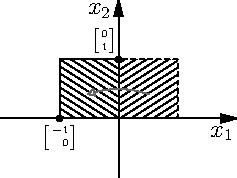
\includegraphics[totalheight=4cm]{symmetry_02}} & $\left[\begin{array}{r r} -1 & 0\\ 0 & 1\end{array}\right]$\\\hline
关于直线$y=x$对称 & \raisebox{0pt}[4.2cm][0.2cm]{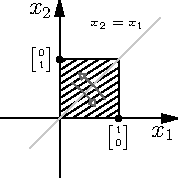
\includegraphics[totalheight=4cm]{symmetry_03}} & $\left[\begin{array}{r r} 0 & 1\\ 1 & 0\end{array}\right]$\\\hline
关于直线$y=-x$对称 & \raisebox{0pt}[4.2cm][0.2cm]{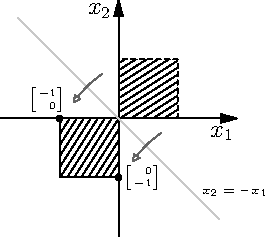
\includegraphics[totalheight=4cm]{symmetry_04}} & $\left[\begin{array}{r r} 0 & -1\\ -1 & 0\end{array}\right]$\\\hline
关于原点对称 & \raisebox{0pt}[4.2cm][0.2cm]{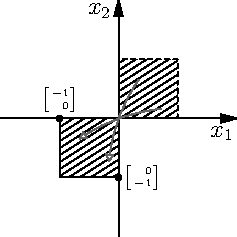
\includegraphics[totalheight=4cm]{symmetry_05}} & $\left[\begin{array}{r r} -1 & 0\\ 0 & -1\end{array}\right]$\\\hline
沿$x$轴拉伸 & \raisebox{0pt}[4.2cm][0.2cm]{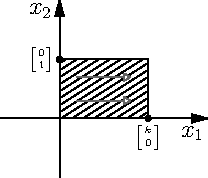
\includegraphics[totalheight=4cm]{scale_01}} & $\left[\begin{array}{r r} k & 0\\ 0 & 1\end{array}\right]$\\\hline
沿$y$轴拉伸 & \raisebox{0pt}[4.2cm][0.2cm]{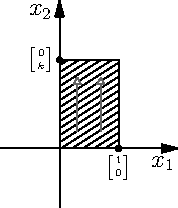
\includegraphics[totalheight=4cm]{scale_02}} & $\left[\begin{array}{r r} 1 & 0\\ 0 & k\end{array}\right]$\\\hline
沿$x$轴倾斜 & \raisebox{0pt}[4.2cm][0.2cm]{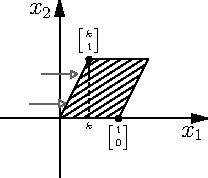
\includegraphics[totalheight=4cm]{slant_01}} & $\left[\begin{array}{r r} 1 & k\\ 0 & 1\end{array}\right]$\\\hline
沿$y$轴倾斜 & \raisebox{0pt}[4.2cm][0.2cm]{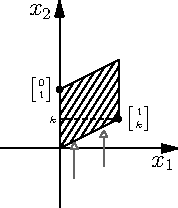
\includegraphics[totalheight=4cm]{slant_02}} & $\left[\begin{array}{r r} 1 & 0\\ k & 1\end{array}\right]$\\\hline
投影到$x$轴 & \raisebox{0pt}[4.2cm][0.2cm]{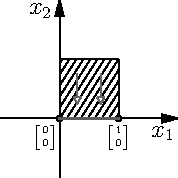
\includegraphics[totalheight=4cm]{shadow_01}} & $\left[\begin{array}{r r} 1 & 0\\ 0 & 0\end{array}\right]$\\\hline
投影到$y$轴 & \raisebox{0pt}[4.2cm][0.2cm]{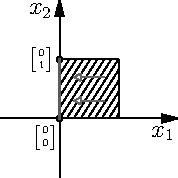
\includegraphics[totalheight=4cm]{shadow_02}} & $\left[\begin{array}{r r} 0 & 0\\ 0 & 1\end{array}\right]$\\\hline
\caption{线性变换一览}
\end{longtable}\vspace{6ex}

\section{商业、科学和工程中的线性模型}
例1. 如表格所示, 代表食谱中的三种食物以及100克每种食物成分含有某些营养素的数量. 求出脱脂牛奶、大豆粉和乳清的某种组合, 使该食谱每天能供给如图表所需的蛋白质、碳水化合物和脂肪的含量.\\
\begin{table}[H]
\begin{tabular}{l c c c c}

\end{tabular}
\end{table}

\begin{law}[基尔霍夫电压定律]\ \\
围绕一条回路同一方向的电压降$RI$的代数和等于围绕该回路的同一方向电动势的代数和.
\end{law}\vspace{4ex}

\begin{law}
如果有矩阵$A$使$\bm{x}_1=A\bm{x}_0$,$\bm{x}_2=A\bm{x}_1$, 一般地,
\[\bm{x}_{k+1}=A\bm{x}_k\text{,\ }k=0,1,2,\cdots\]
则称为\textbf{线性差分方程}(或\textbf{递归关系}).
\end{law}
